\begin{figure*}
    \begin{subfigure}[b]{0.25\textwidth}
        \centering
<<<<<<< HEAD
        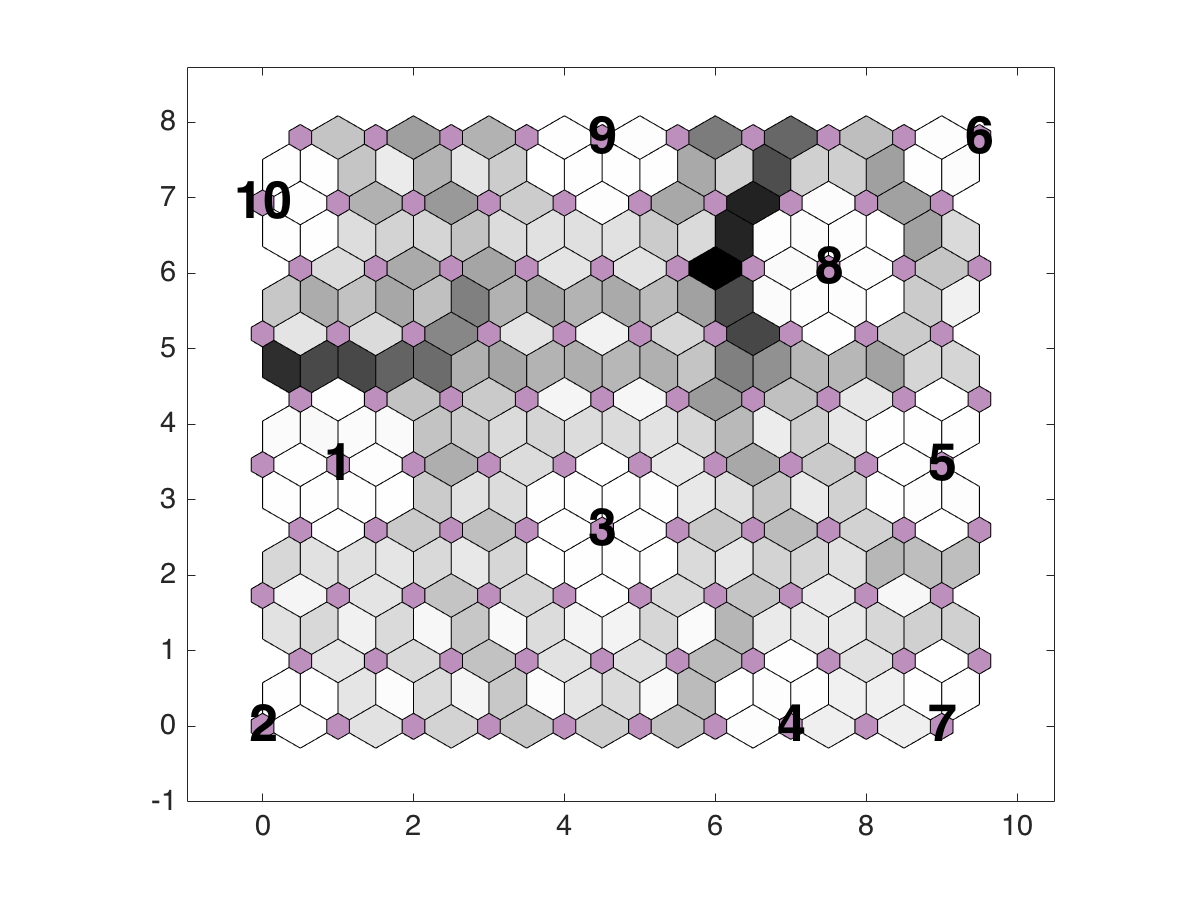
\includegraphics[width=54mm, height=38mm]{../../images0.01/M31/2D/diff_dimension/combine_2D_data_between_cols3and11.png}
=======
        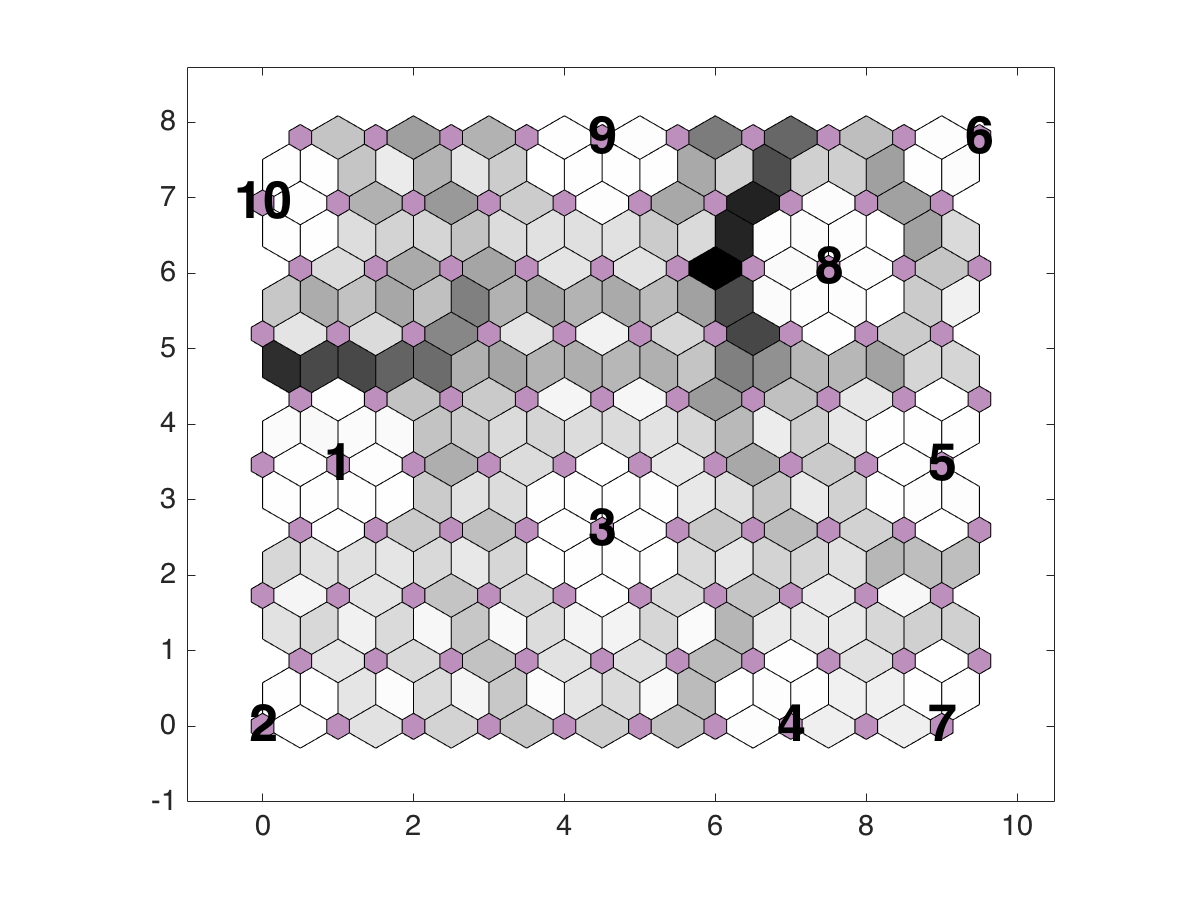
\includegraphics[width=54mm, height=37mm]{../../images0.01/M31/2D/diff_dimension/combine_2D_data_between_cols3and11.png}
>>>>>>> sharelatex-2016-07-26-1530
        \caption{Input data: data from Fig.~\ref{fig: only_pahs} and \halpha}
        \label{fig: col3and11_dist}
    \end{subfigure}
    \hfill
    \begin{subfigure}[b]{0.25\textwidth}
        \centering
<<<<<<< HEAD
        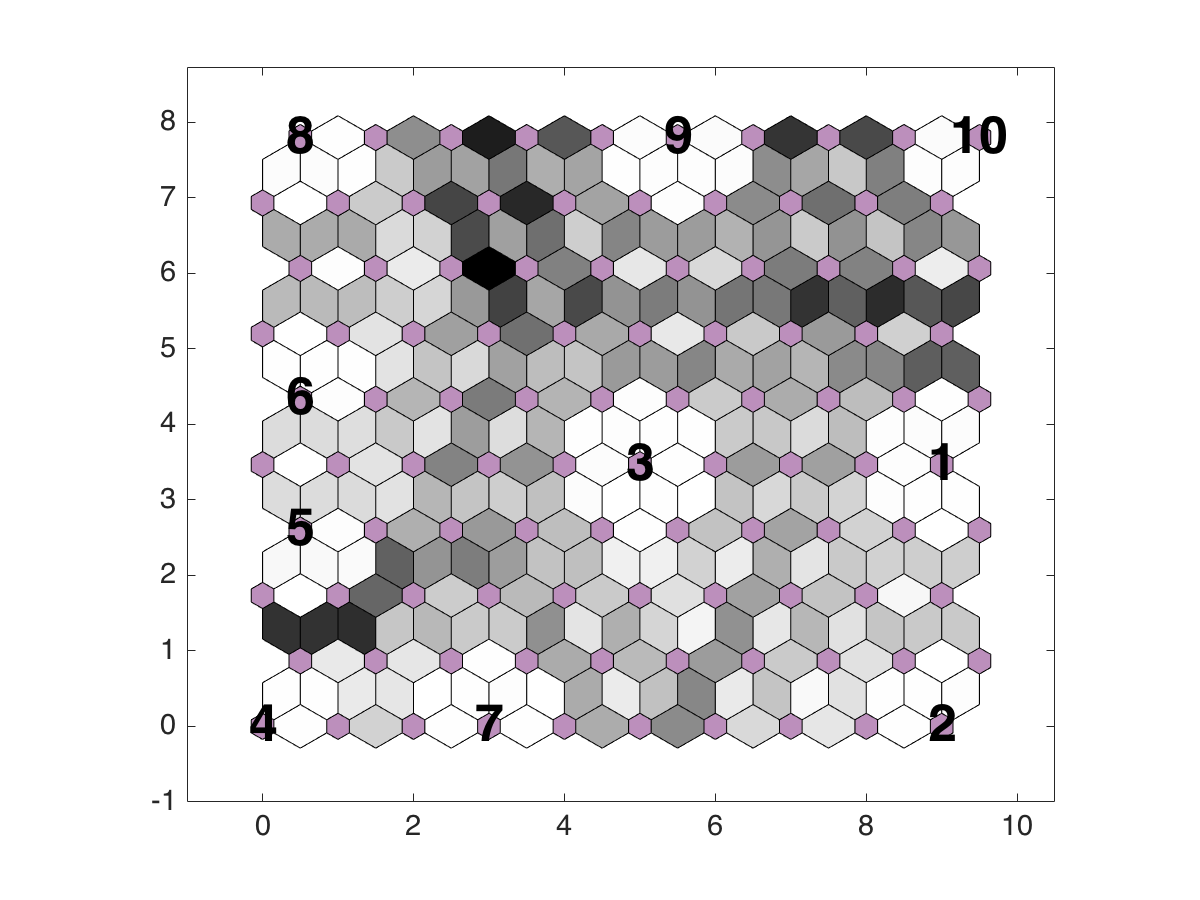
\includegraphics[width=54mm, height=38mm]{../../images0.01/M31/2D/diff_dimension/combine_2D_data_between_cols3and12.png}
=======
        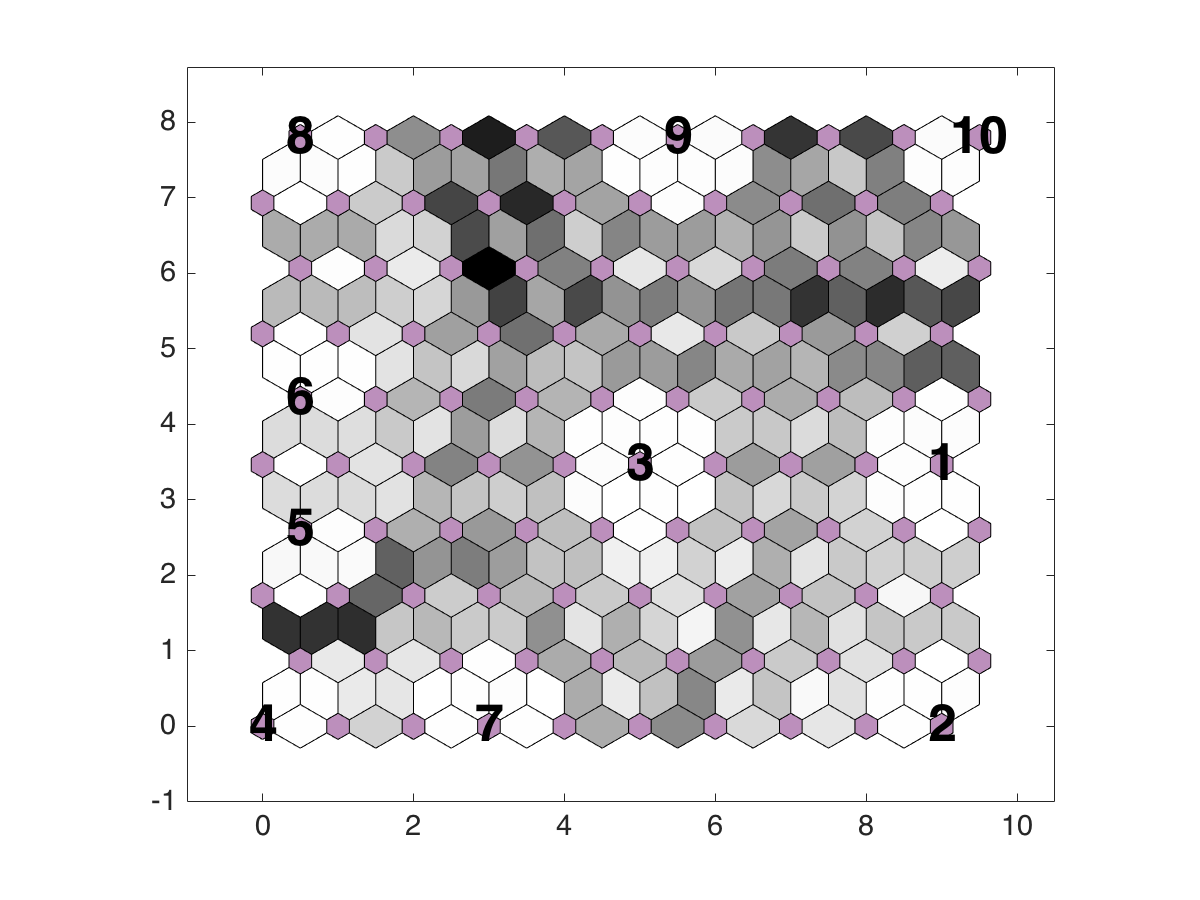
\includegraphics[width=54mm, height=37mm]{../../images0.01/M31/2D/diff_dimension/combine_2D_data_between_cols3and12.png}
>>>>>>> sharelatex-2016-07-26-1530
        \caption{Input data: data from Fig.~\ref{fig: col3and11_dist} and \oiii}
        \label{fig: col3and12_dist}
    \end{subfigure}
        \hfill
    \begin{subfigure}[b]{0.25\textwidth}
        \centering
<<<<<<< HEAD
        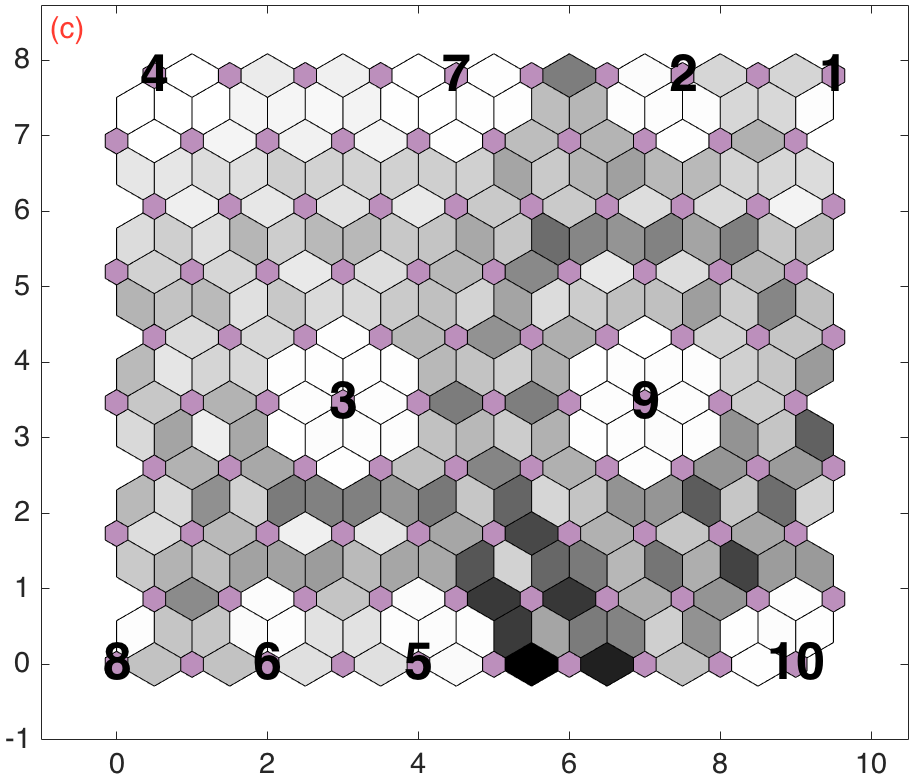
\includegraphics[width=54mm, height=38mm]{../../images0.01/M31/2D/diff_dimension/combine_2D_data_between_cols3and13.png}
=======
        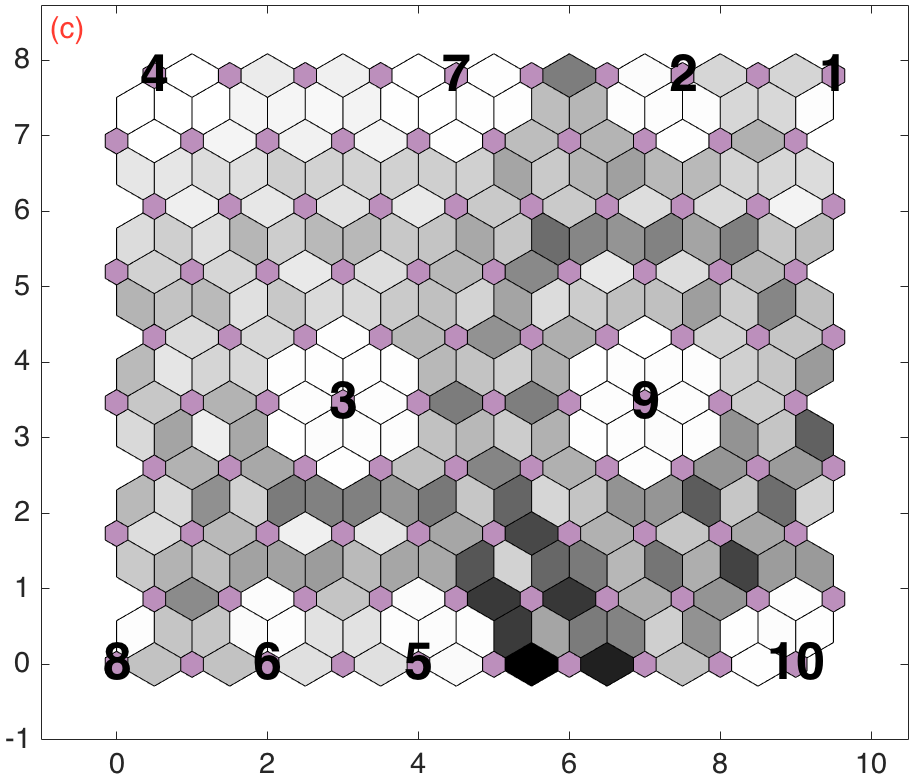
\includegraphics[width=54mm, height=37mm]{../../images0.01/M31/2D/diff_dimension/combine_2D_data_between_cols3and13.png}
>>>>>>> sharelatex-2016-07-26-1530
        \caption{Input data: data from Fig.~\ref{fig: col3and12_dist} and \sii}
        \label{fig: col3and13_dist}
    \end{subfigure}
        \hfill
    \begin{subfigure}[b]{0.25\textwidth}
        \centering
<<<<<<< HEAD
        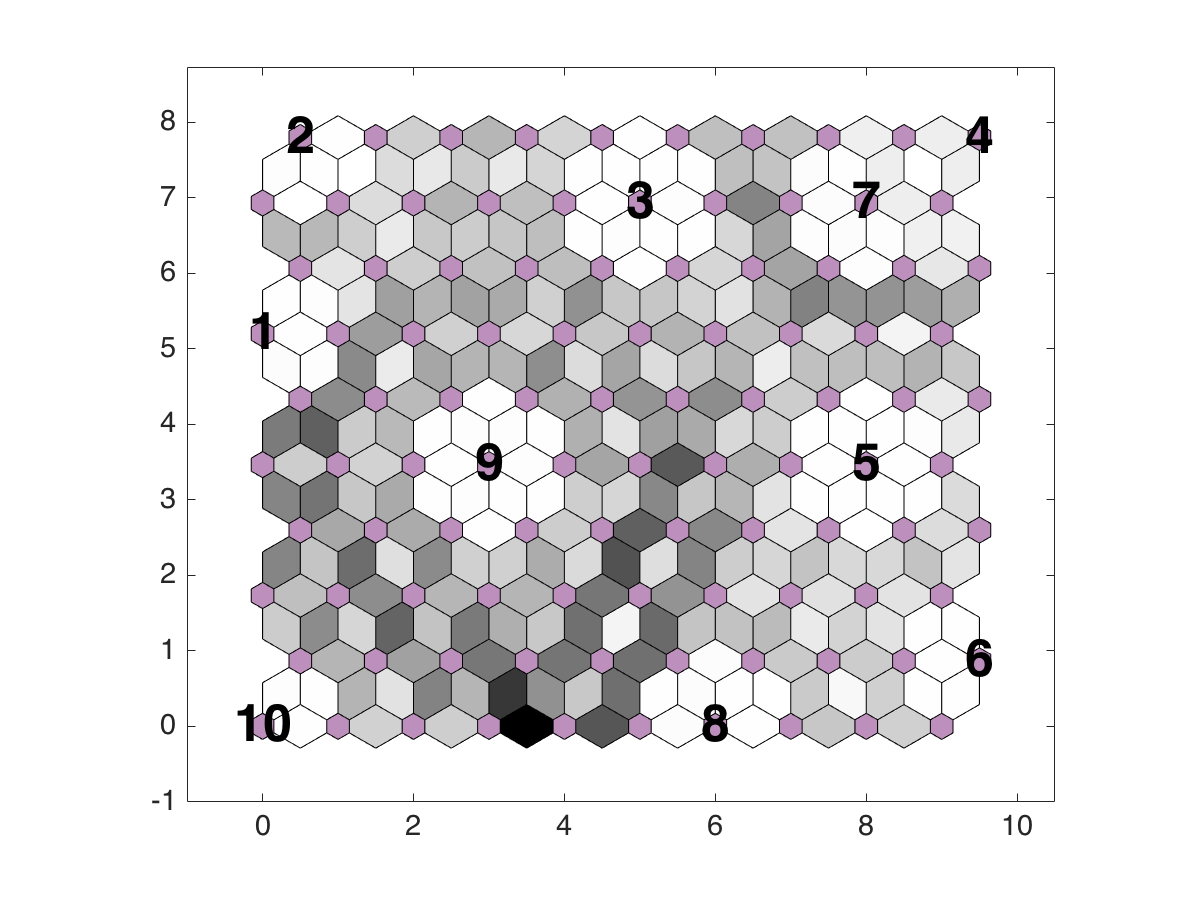
\includegraphics[width=54mm, height=38mm]{../../images0.01/M31/2D/diff_dimension/combine_2D_data_between_cols3and14.png}
=======
        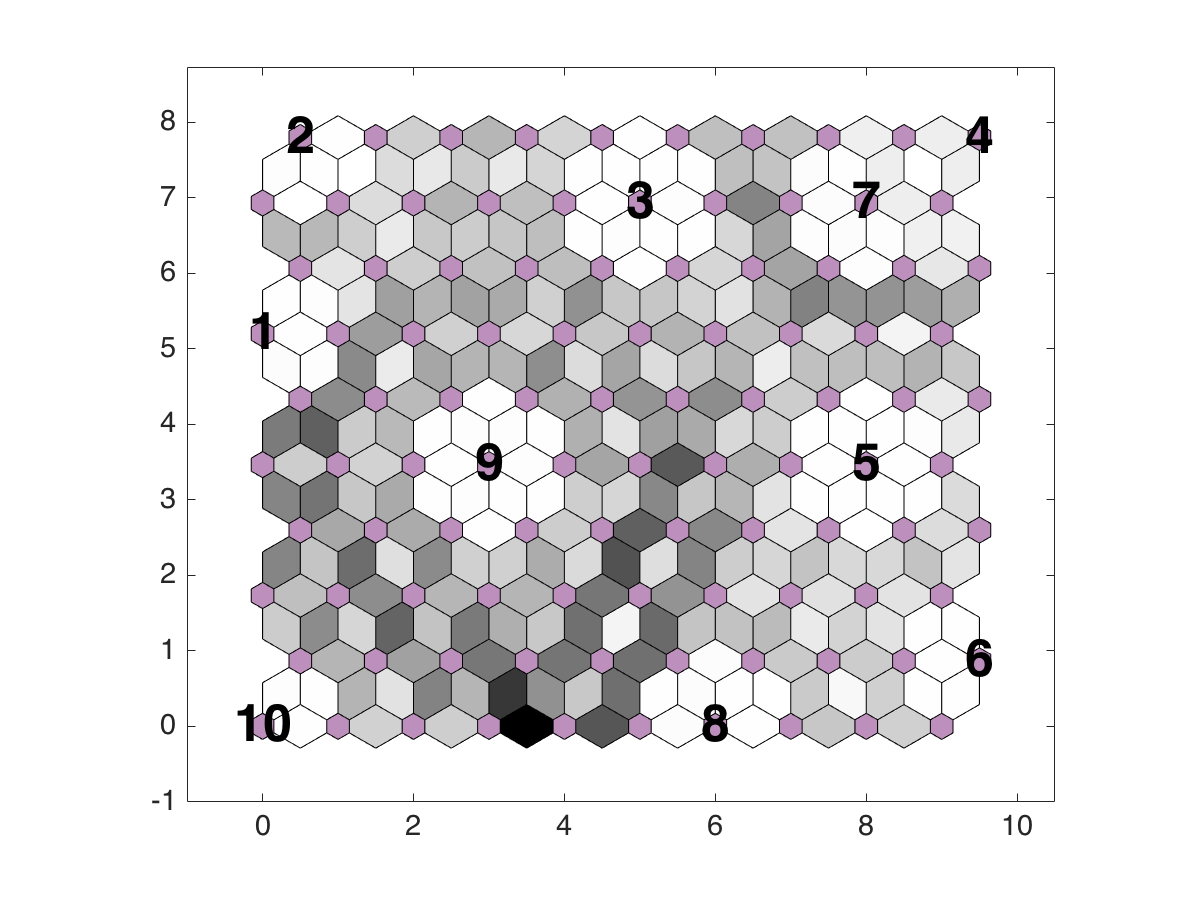
\includegraphics[width=54mm, height=37mm]{../../images0.01/M31/2D/diff_dimension/combine_2D_data_between_cols3and14.png}
>>>>>>> sharelatex-2016-07-26-1530
        \caption{Input data: data from Fig.~\ref{fig: col3and13_dist} and IRAC~5.7~$\mu$m emission}
        \label{fig: col3and14_dist}
    \end{subfigure}
        \hfill
    \begin{subfigure}[b]{0.25\textwidth}
        \centering
<<<<<<< HEAD
        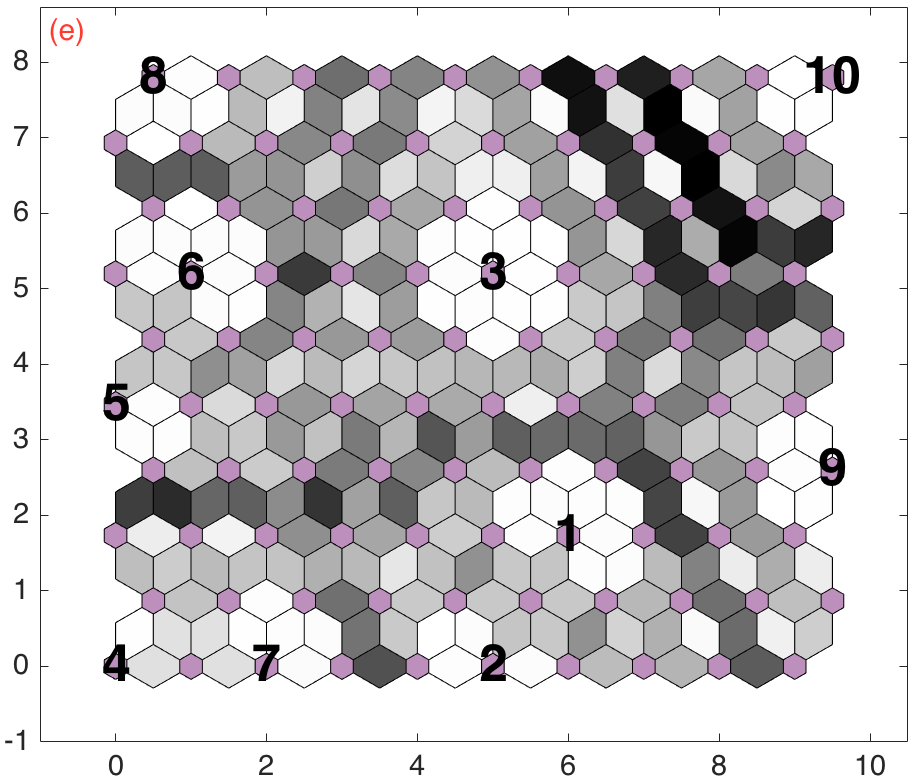
\includegraphics[width=54mm, height=38mm]{../../images0.01/M31/2D/diff_dimension/combine_2D_data_between_cols3and15.png}
=======
        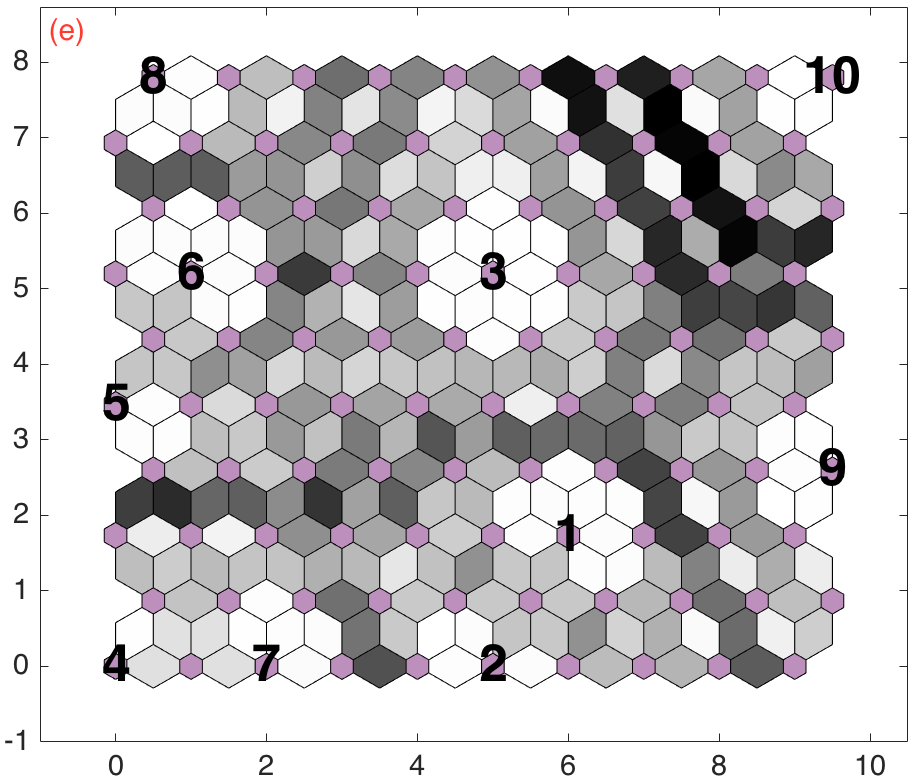
\includegraphics[width=54mm, height=37mm]{../../images0.01/M31/2D/diff_dimension/combine_2D_data_between_cols3and15.png}
>>>>>>> sharelatex-2016-07-26-1530
        \caption{Input data: data from Fig.~\ref{fig: col3and14_dist} and PACS~100~$\mu$m emission }
        \label{fig: col3and15_dist}
    \end{subfigure}
        \hfill
    \begin{subfigure}[b]{0.25\textwidth}
        \centering
<<<<<<< HEAD
        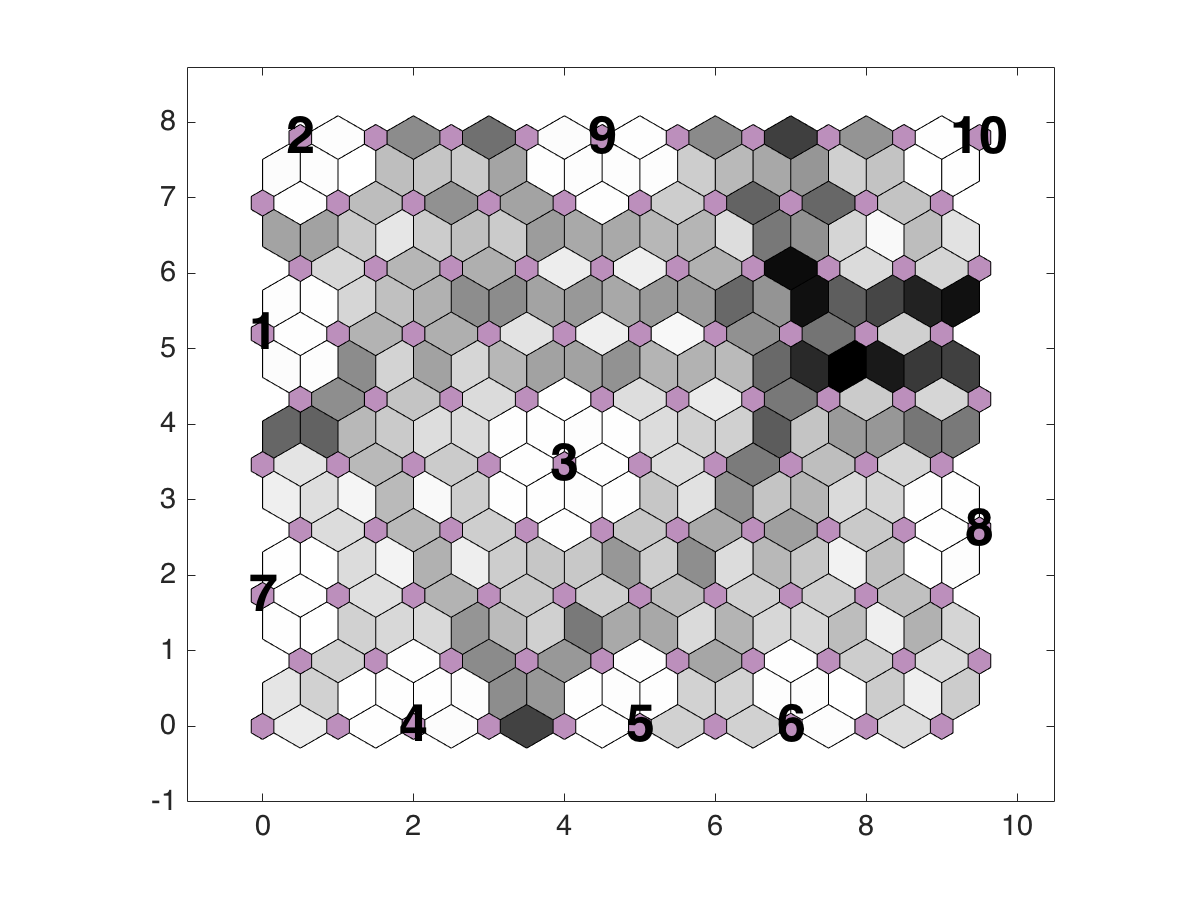
\includegraphics[width=54mm, height=38mm]{../../images0.01/M31/2D/diff_dimension/combine_2D_data_between_cols3and16.png}
=======
        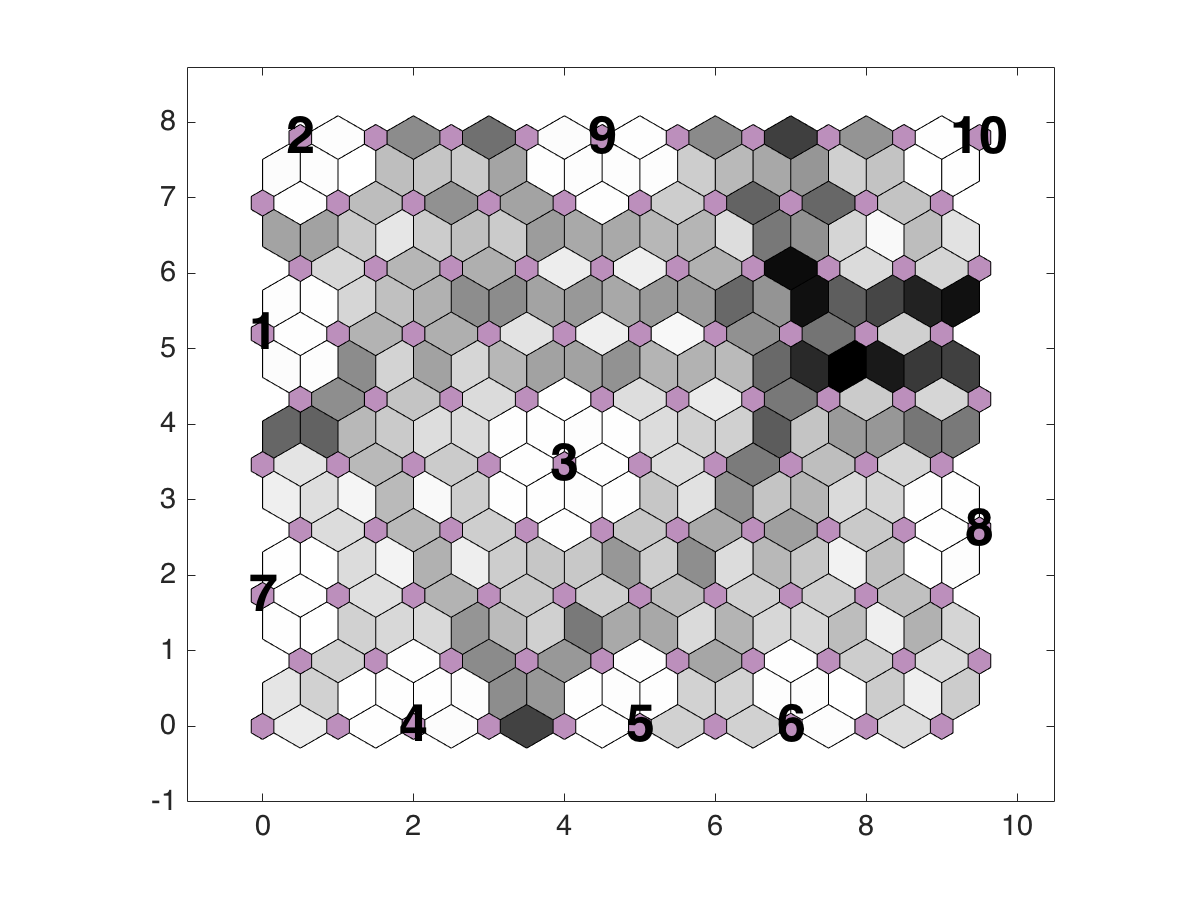
\includegraphics[width=54mm, height=37mm]{../../images0.01/M31/2D/diff_dimension/combine_2D_data_between_cols3and16.png}
>>>>>>> sharelatex-2016-07-26-1530
        \caption{Input data: data from Fig.~\ref{fig: col3and15_dist} and SPIRE~250~$\mu$m emission }
        \label{fig: col3and16_dist}
    \end{subfigure}
        \hfill
    \begin{subfigure}[b]{0.25\textwidth}
        \centering
<<<<<<< HEAD
        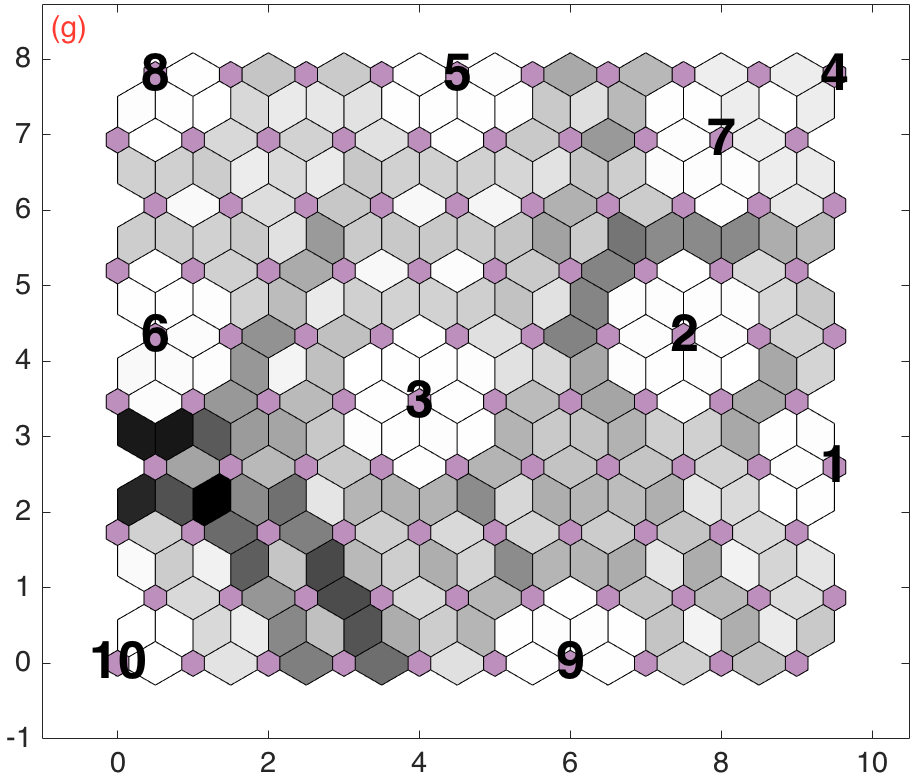
\includegraphics[width=54mm, height=38mm]{../../images0.01/M31/2D/diff_dimension/combine_2D_data_between_cols3and17.png}
=======
        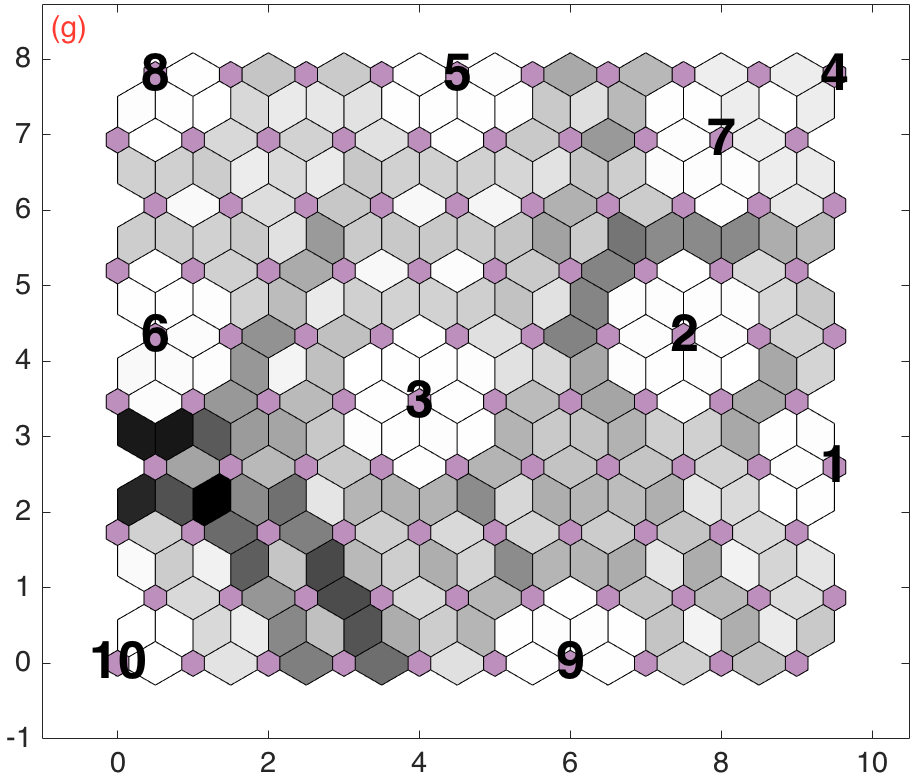
\includegraphics[width=54mm, height=37mm]{../../images0.01/M31/2D/diff_dimension/combine_2D_data_between_cols3and17.png}
>>>>>>> sharelatex-2016-07-26-1530
        \caption{Input data: data from Fig.~\ref{fig: col3and16_dist} and SPIRE~350~$\mu$m emission }
        \label{fig: col3and17_dist}
    \end{subfigure}
        \hfill
    \begin{subfigure}[b]{0.25\textwidth}
        \centering
<<<<<<< HEAD
        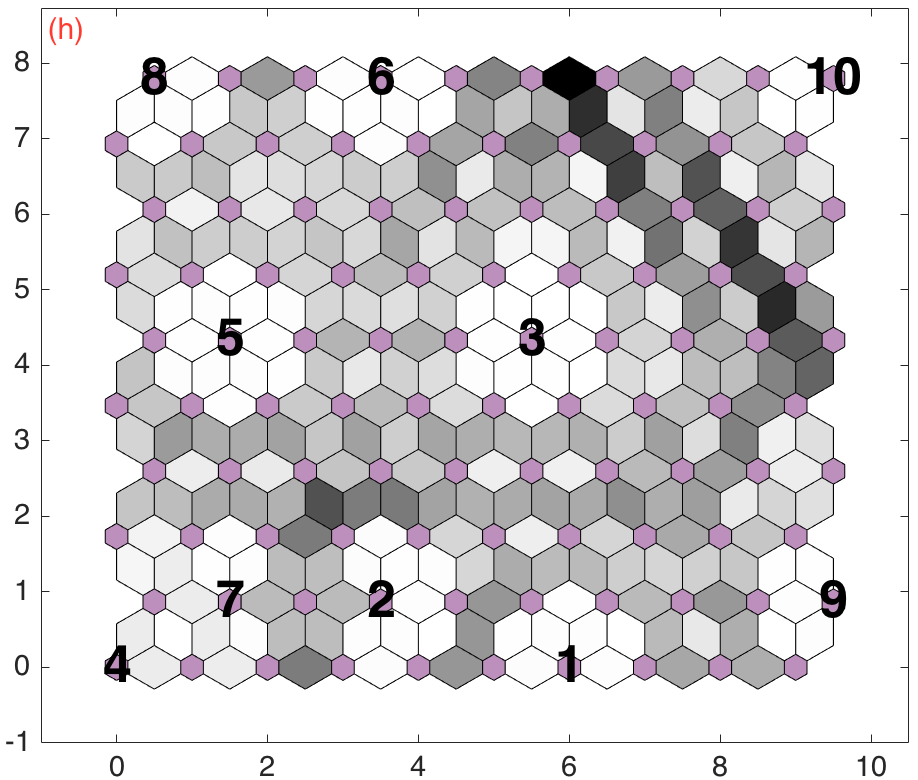
\includegraphics[width=54mm, height=38mm]{../../images0.01/M31/2D/diff_dimension/combine_2D_data_between_cols3and18.png}
=======
        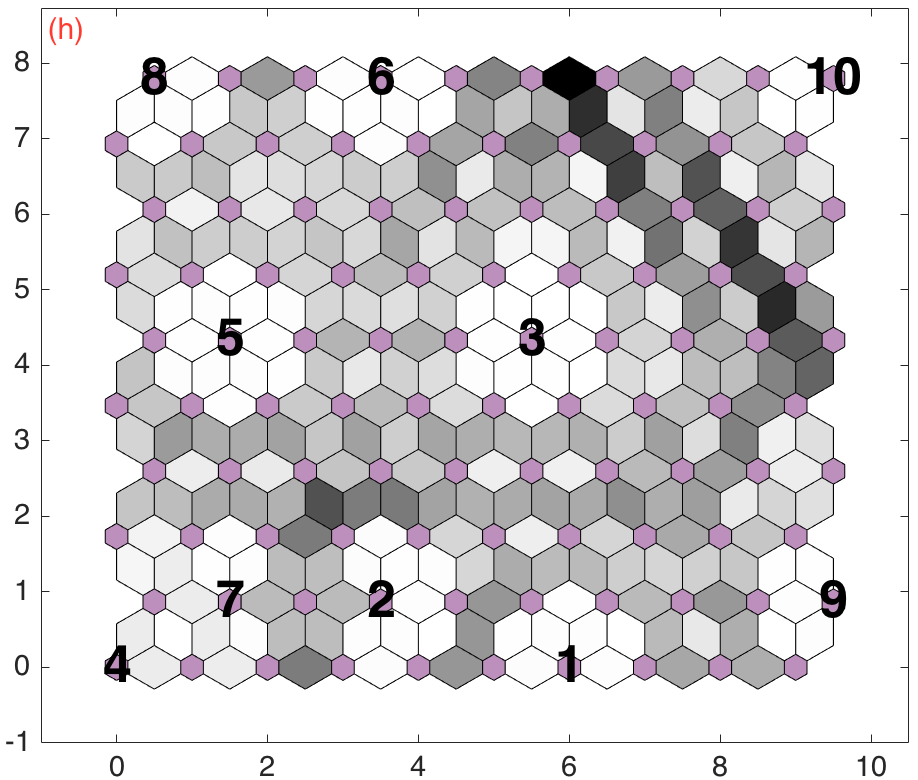
\includegraphics[width=54mm, height=37mm]{../../images0.01/M31/2D/diff_dimension/combine_2D_data_between_cols3and18.png}
>>>>>>> sharelatex-2016-07-26-1530
        \caption{Input data: data from Fig.~\ref{fig: col3and17_dist} and SPIRE~500~$\mu$m emission }
        \label{fig: col3and18_dist}
    \end{subfigure}
        \hfill
    \begin{subfigure}[b]{0.25\textwidth}
        \centering
<<<<<<< HEAD
        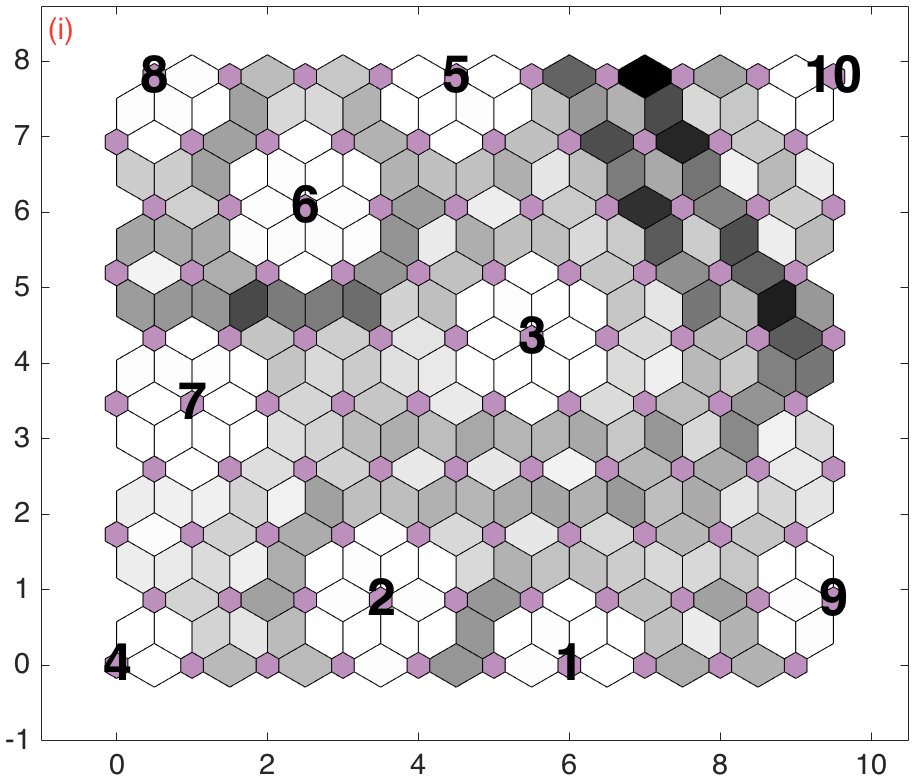
\includegraphics[width=54mm, height=38mm]{../../images0.01/M31/2D/diff_dimension/combine_2D_data_between_cols3and19.png}
=======
        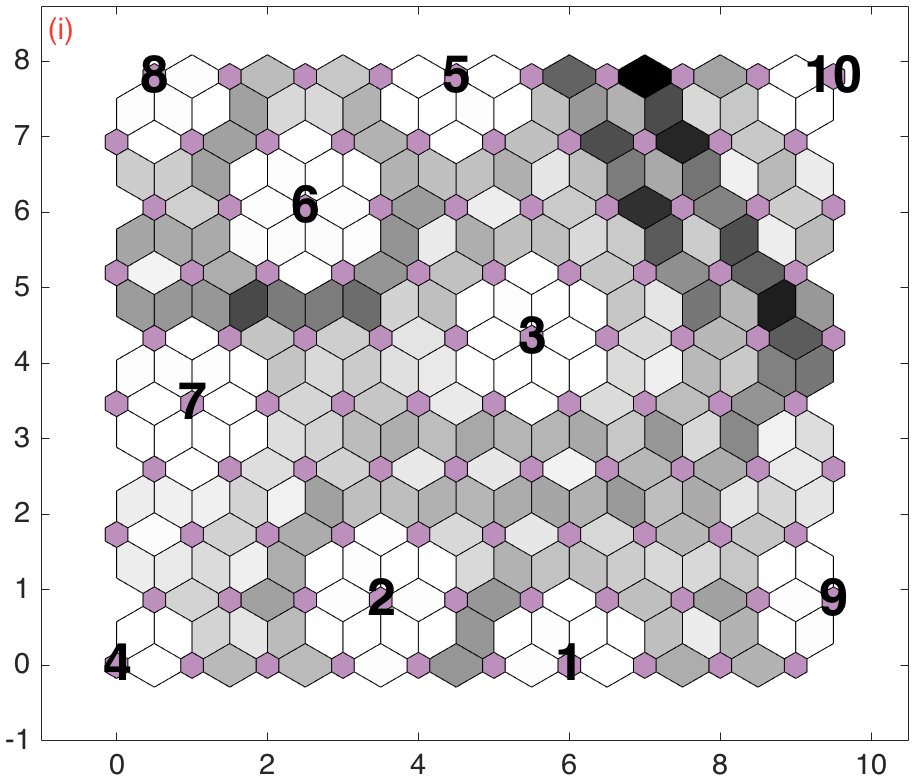
\includegraphics[width=54mm, height=37mm]{../../images0.01/M31/2D/diff_dimension/combine_2D_data_between_cols3and19.png}
>>>>>>> sharelatex-2016-07-26-1530
         \caption{Input data: data from Fig.~\ref{fig: col3and18_dist} and L$_{{\mathrm Dust}}$}
        \label{fig: col3and19_dist}
    \end{subfigure}
        \hfill
    \begin{subfigure}[b]{0.25\textwidth}
        \centering
<<<<<<< HEAD
        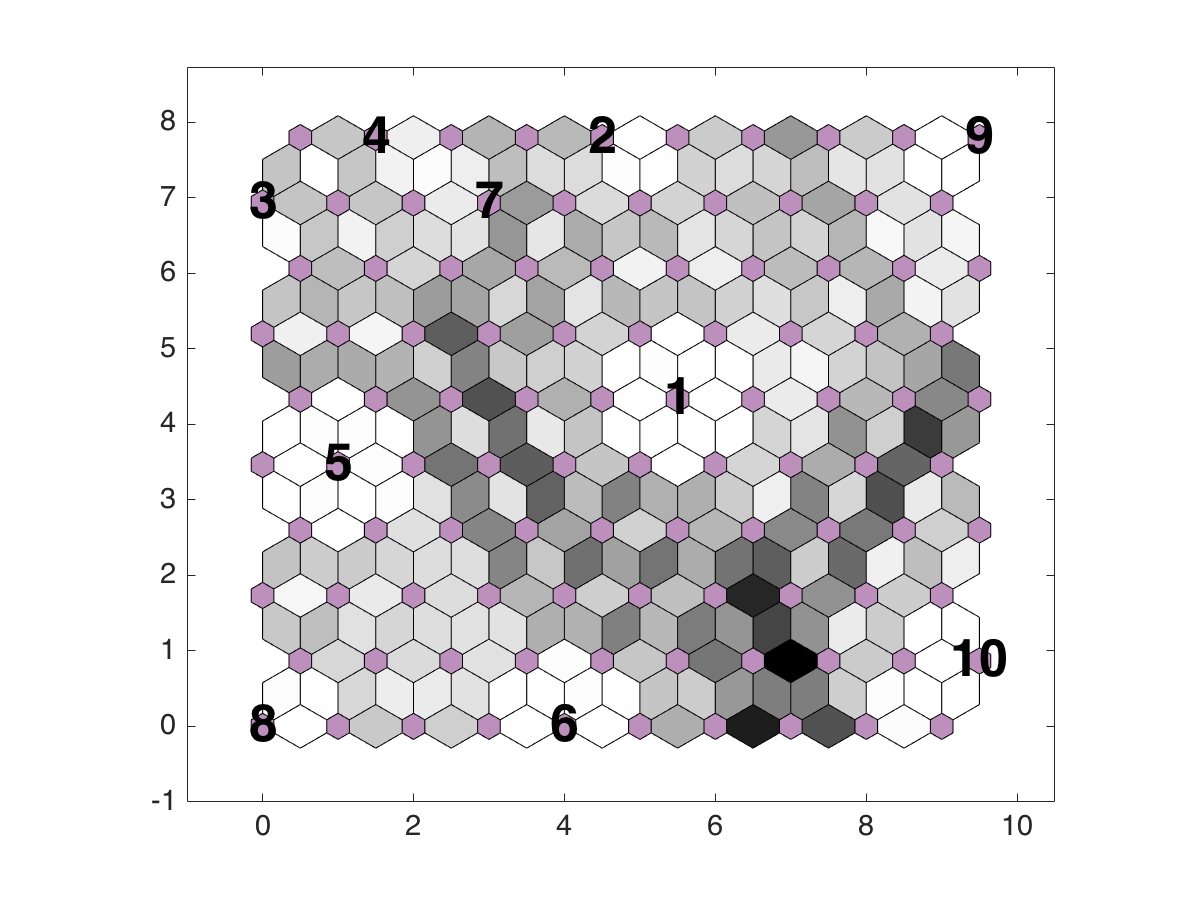
\includegraphics[width=54mm, height=38mm]{../../images0.01/M31/2D/diff_dimension/combine_2D_data_between_cols3and20.png}
=======
        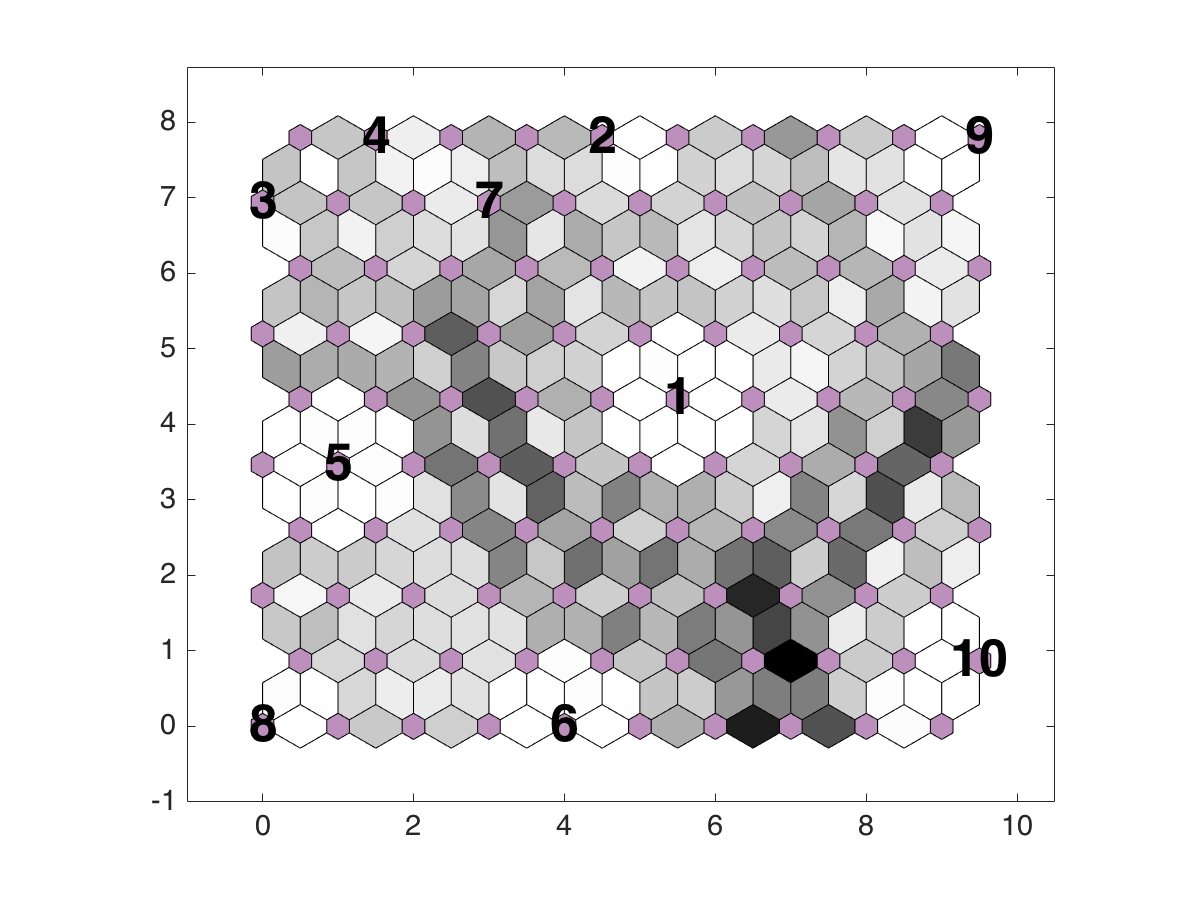
\includegraphics[width=54mm, height=37mm]{../../images0.01/M31/2D/diff_dimension/combine_2D_data_between_cols3and20.png}
>>>>>>> sharelatex-2016-07-26-1530
          \caption{Input data: data from Fig.~\ref{fig: col3and19_dist} and M$_{{\mathrm Dust}}$}
        \label{fig: col3and20_dist}
    \end{subfigure}        \hfill
    \begin{subfigure}[b]{0.25\textwidth}
        \centering
<<<<<<< HEAD
        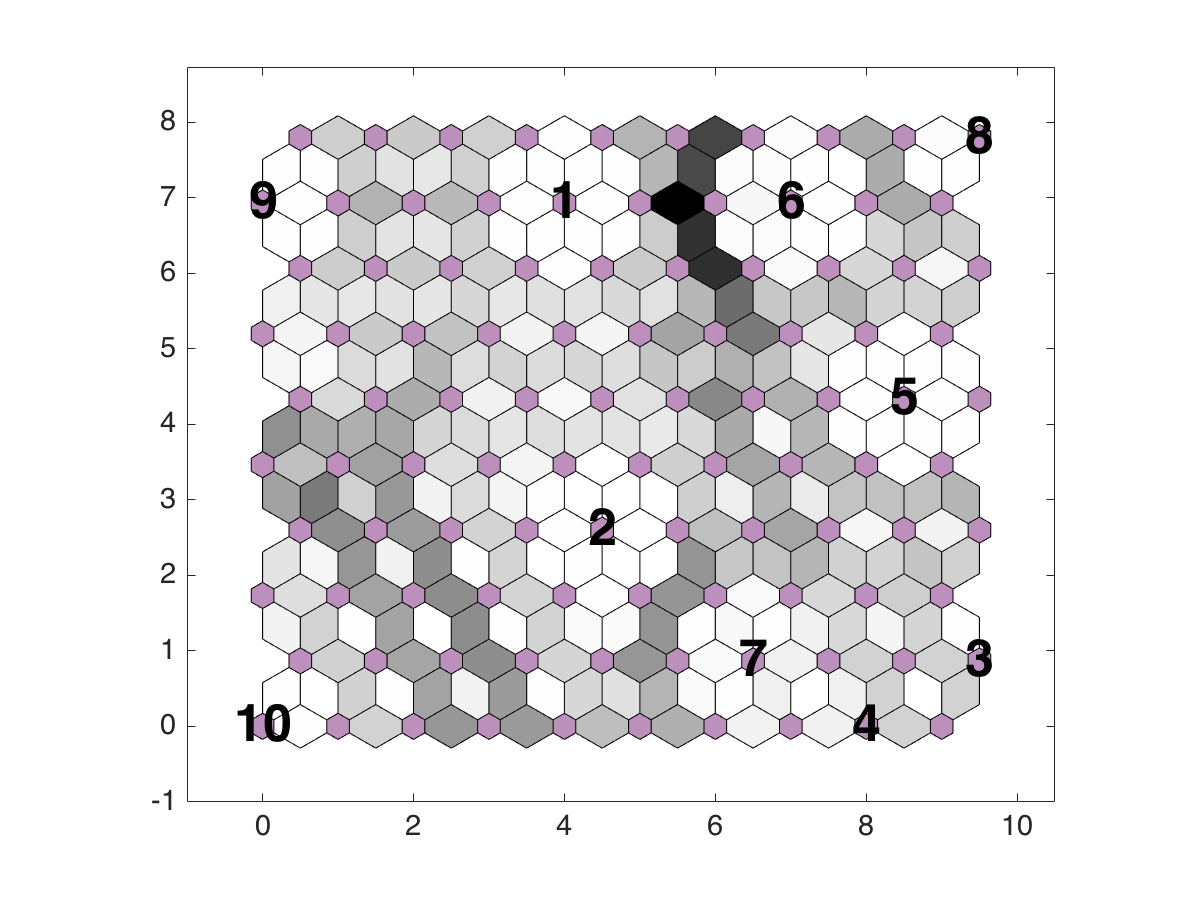
\includegraphics[width=54mm, height=38mm]{../../images0.01/M31/2D/diff_dimension/combine_2D_data_between_cols3and21.png}
        \caption{Input data: data from Fig.~\ref{fig: col3and20_dist} and SFR}
=======
        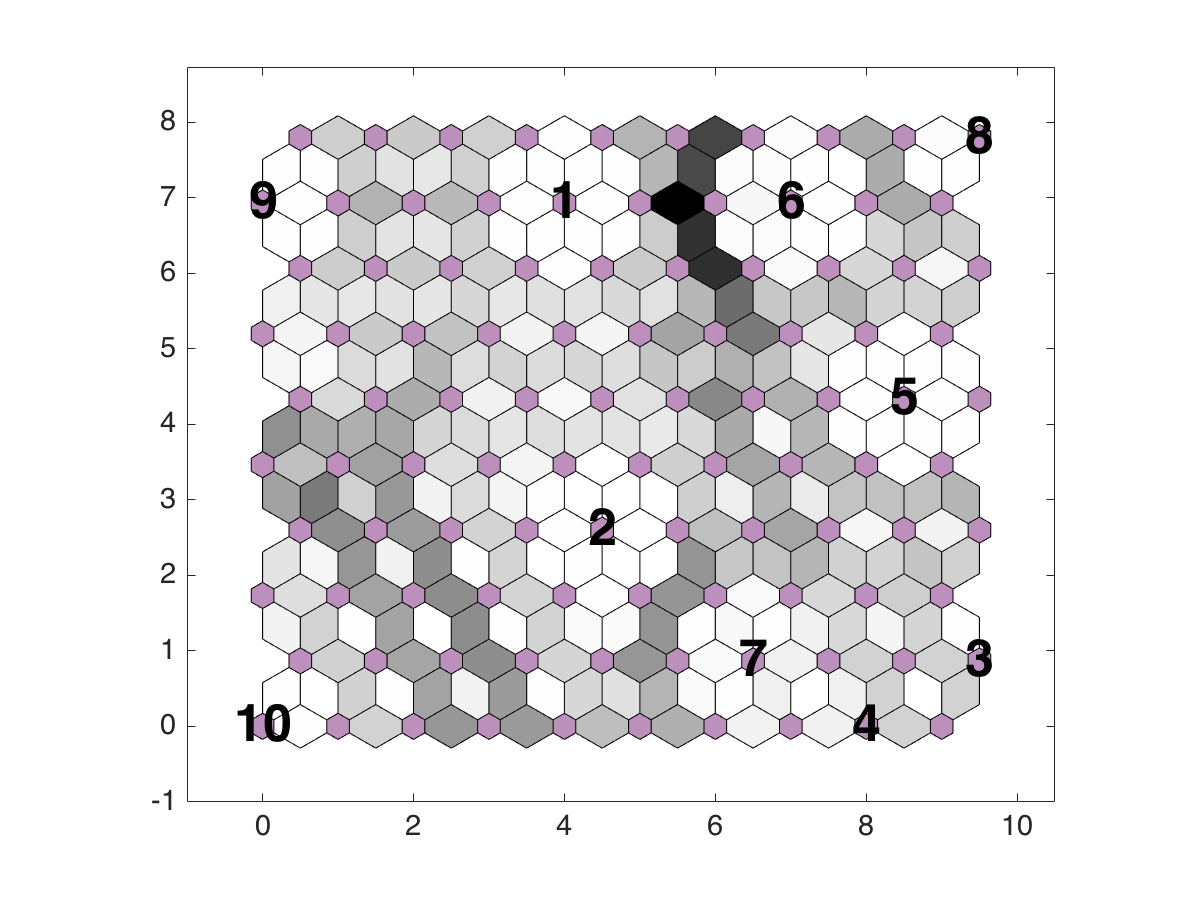
\includegraphics[width=54mm, height=37mm]{../../images0.01/M31/2D/diff_dimension/combine_2D_data_between_cols3and21.png}
        \caption{Input data: data from Fig.~\ref{fig: col3and20_dist} and SFR(FUV\ +\ 24\ $\mu$m)}
>>>>>>> sharelatex-2016-07-26-1530
        \label{fig: col3and21_dist}
    \end{subfigure}
            \hfill
    \begin{subfigure}[b]{0.25\textwidth}
        \centering
<<<<<<< HEAD
        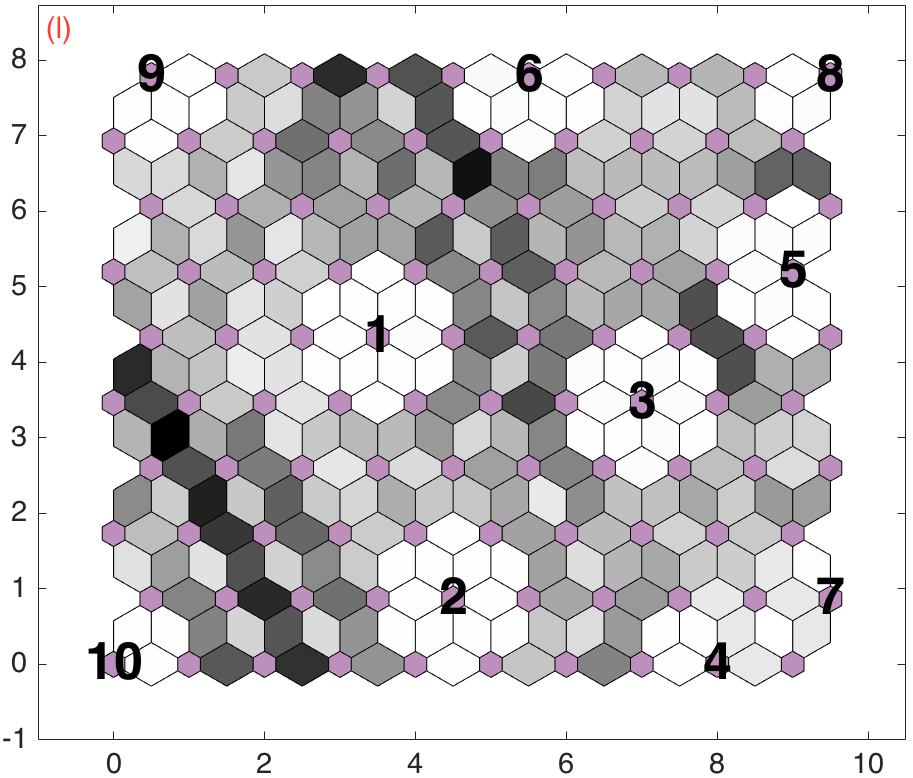
\includegraphics[width=54mm, height=38mm]{../../images0.01/M31/2D/diff_dimension/combine_2D_data_between_cols3and22.png}
=======
        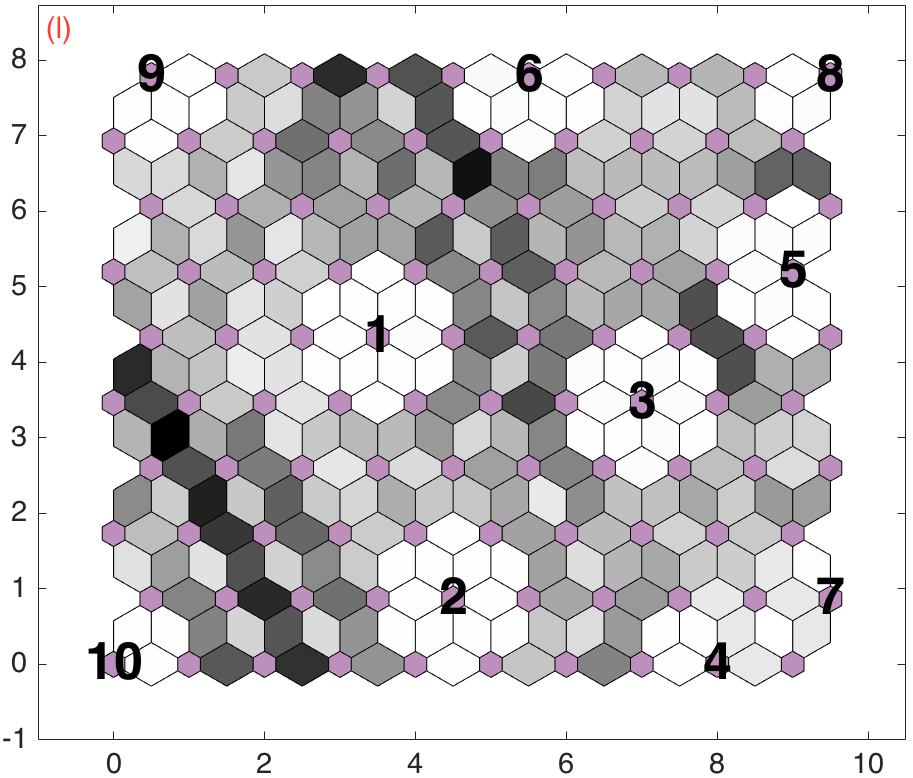
\includegraphics[width=54mm, height=37mm]{../../images0.01/M31/2D/diff_dimension/combine_2D_data_between_cols3and22.png}
>>>>>>> sharelatex-2016-07-26-1530
        \caption{Input data: data from Fig.~\ref{fig: col3and21_dist} and M$_{{\mathrm Stars}}$}
        \label{fig: col3and22_dist}
    \end{subfigure}
            \hfill
    \begin{subfigure}[b]{0.25\textwidth}
        \centering
<<<<<<< HEAD
        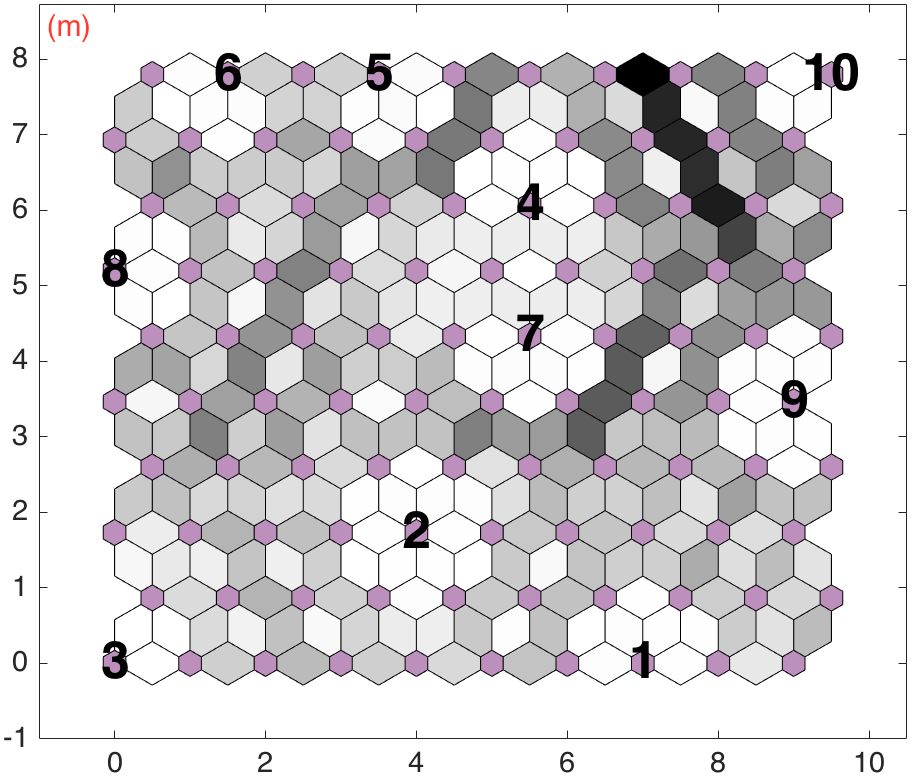
\includegraphics[width=54mm, height=38mm]{../../images0.01/M31/2D/diff_dimension/combine_2D_data_between_cols3and23.png}
=======
        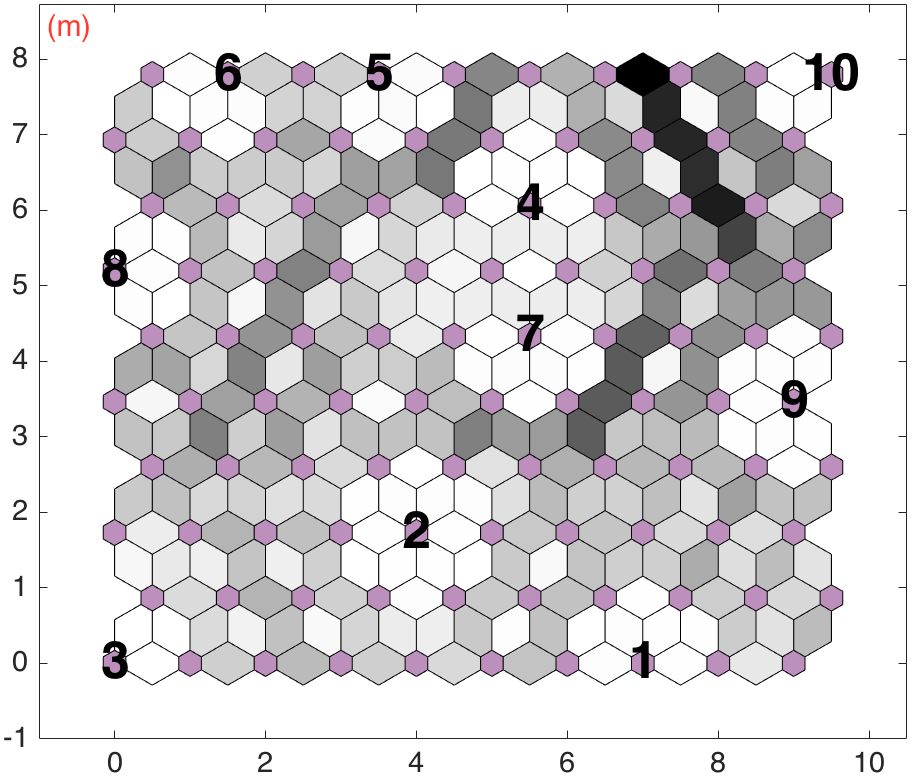
\includegraphics[width=54mm, height=37mm]{../../images0.01/M31/2D/diff_dimension/combine_2D_data_between_cols3and23.png}
>>>>>>> sharelatex-2016-07-26-1530
        \caption{Input data: data from Fig.~\ref{fig: col3and22_dist} and L$_{{\mathrm TIR}}$}
        \label{fig: col3and23_dist}
    \end{subfigure}
            \hfill
    \begin{subfigure}[b]{0.25\textwidth}
        \centering
<<<<<<< HEAD
        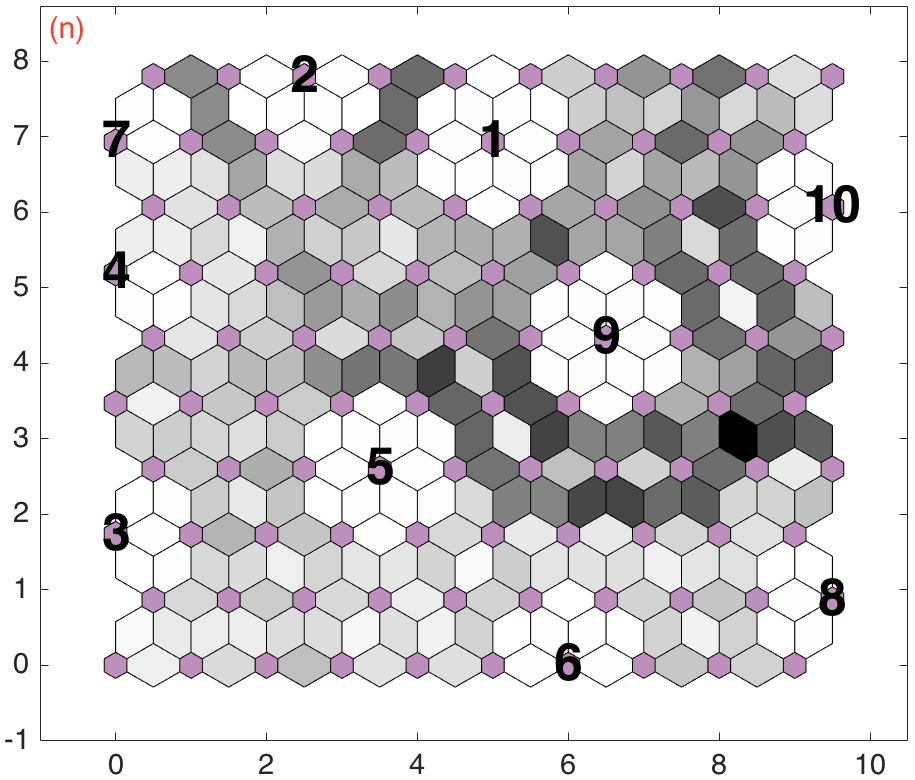
\includegraphics[width=54mm, height=38mm]{../../images0.01/M31/2D/diff_dimension/combine_2D_data_between_cols3and24.png}
        \caption{Input data: data from Fig.~\ref{fig: col3and23_dist} and M$_{{\mathrm Total gas}}$}
=======
        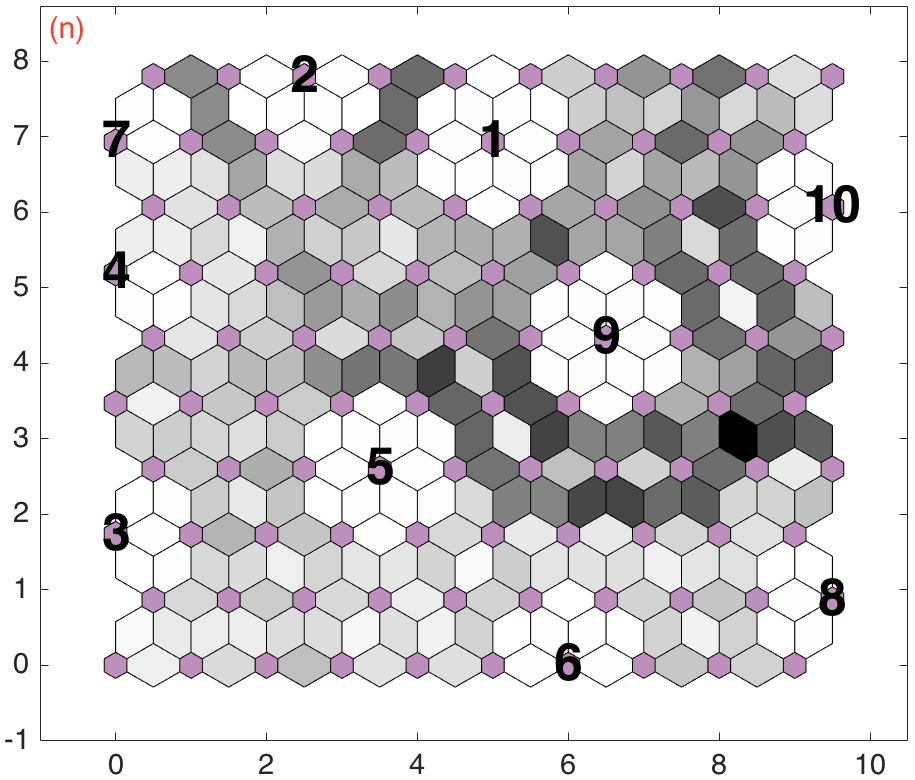
\includegraphics[width=54mm, height=37mm]{../../images0.01/M31/2D/diff_dimension/combine_2D_data_between_cols3and24.png}
        \caption{Input data: data from Fig.~\ref{fig: col3and23_dist} and M$_{{\mathrm Total\ gas}}$}
>>>>>>> sharelatex-2016-07-26-1530
        \label{fig: col3and24_dist}
    \end{subfigure}
            \hfill
    \begin{subfigure}[b]{0.25\textwidth}
        \centering
<<<<<<< HEAD
        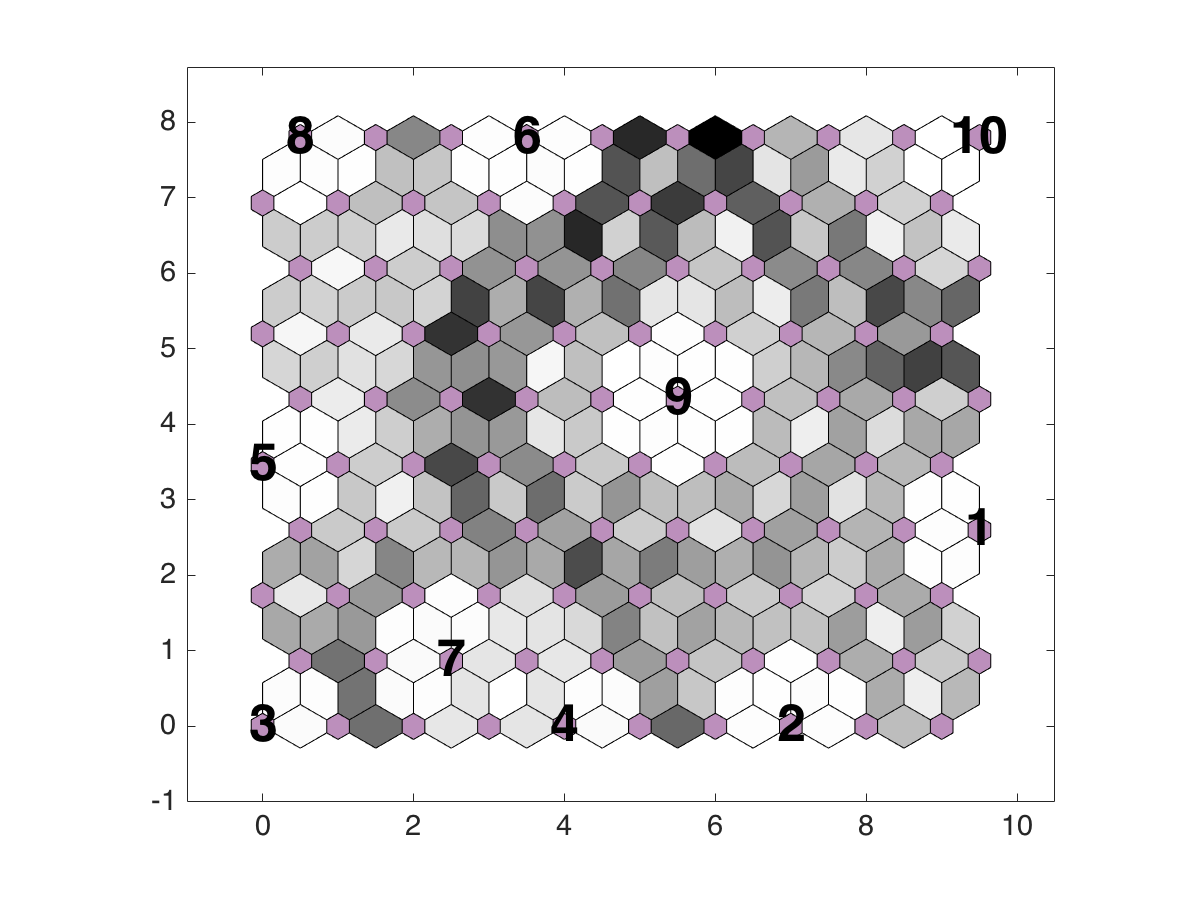
\includegraphics[width=54mm, height=38mm ]{../../images0.01/M31/2D/diff_dimension/combine_2D_data_between_cols3and25.png}
        \caption{Input data: data from Fig.~\ref{fig: col3and19_dist} and M$_{{\mathrm RHI}}$}
        \label{fig: col3and25_dist}
    \end{subfigure}
    \caption{Similar to Fig.~\ref{fig: all_derived_ones}, the result from gradually increasing the dimension of the input data from Fig.~\ref{fig: only_pahs} to 25. The order of the input data is the same as the order in Fig.~\ref{fig: cor_cluster1}.}
=======
        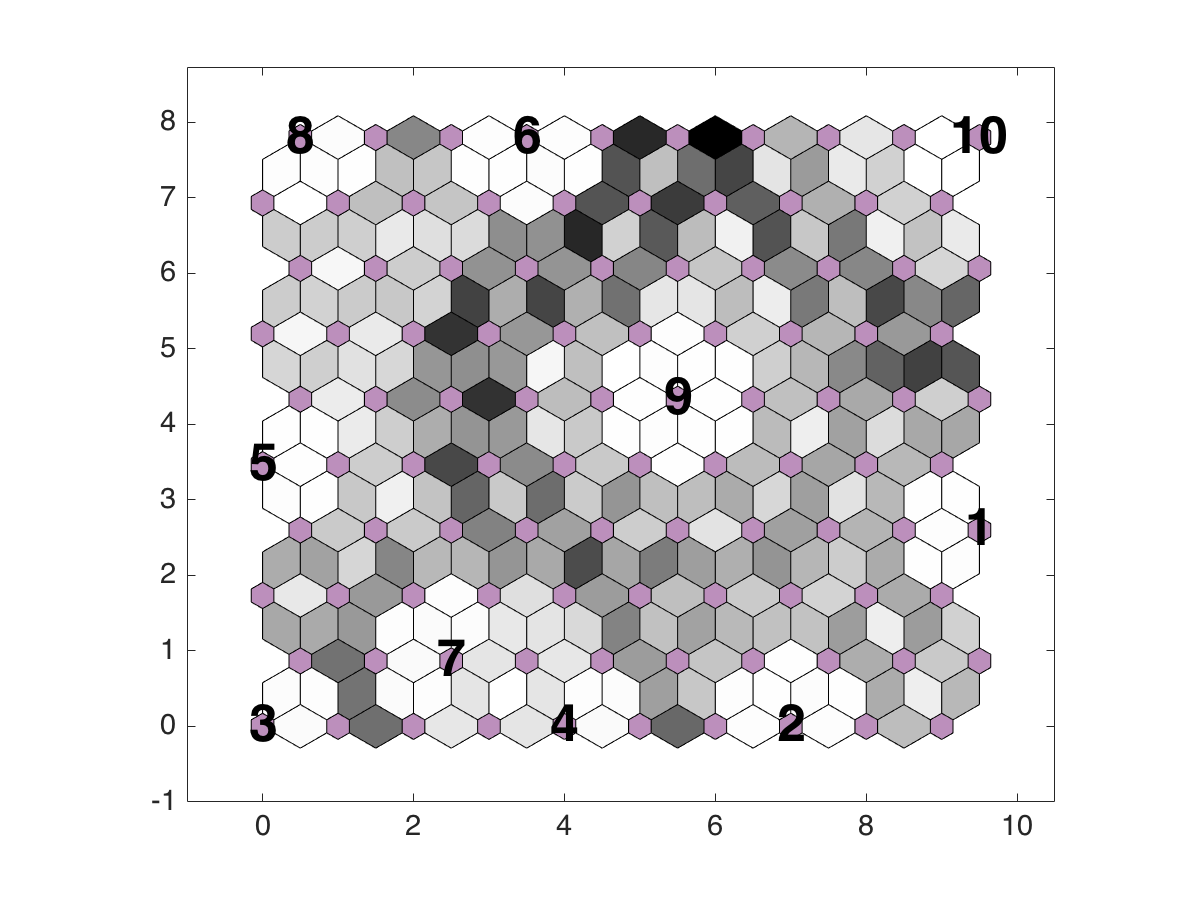
\includegraphics[width=54mm, height=37mm ]{../../images0.01/M31/2D/diff_dimension/combine_2D_data_between_cols3and25.png}
        \caption{Input data: data from Fig.~\ref{fig: col3and19_dist} and RHI.}
        \label{fig: col3and25_dist}
    \end{subfigure}
    \caption{Similar to Fig.~\ref{fig: all_derived_ones}, here we show the result from increasing dimension of input data from Fig.~\ref{fig: only_pahs} to 25, gradually. The order of input data is the same as the order of data in Fig.~\ref{fig: cor_cluster1}.}
>>>>>>> sharelatex-2016-07-26-1530
    \label{fig: inc_D_col3s}
\end{figure*}
